%% 
%% Copyright 2007-2020 Elsevier Ltd
%% 
%% This file is part of the 'Elsarticle Bundle'.
%% ---------------------------------------------
%% 
%% It may be distributed under the conditions of the LaTeX Project Public
%% License, either version 1.2 of this license or (at your option) any
%% later version.  The latest version of this license is in
%%    http://www.latex-project.org/lppl.txt
%% and version 1.2 or later is part of all distributions of LaTeX
%% version 1999/12/01 or later.
%% 
%% The list of all files belonging to the 'Elsarticle Bundle' is
%% given in the file `manifest.txt'.
%% 
%% Template article for Elsevier's document class `elsarticle'
%% with harvard style bibliographic references

%\documentclass[preprint,12pt,authoryear]{elsarticle}

%% Use the option review to obtain double line spacing
%% \documentclass[authoryear,preprint,review,12pt]{elsarticle}

%% Use the options 1p,twocolumn; 3p; 3p,twocolumn; 5p; or 5p,twocolumn
%% for a journal layout:
%% \documentclass[final,1p,times,authoryear]{elsarticle}
%% \documentclass[final,1p,times,twocolumn,authoryear]{elsarticle}
%% \documentclass[final,3p,times,authoryear]{elsarticle}
%% \documentclass[final,3p,times,twocolumn,authoryear]{elsarticle}
%% \documentclass[final,5p,times,authoryear]{elsarticle}
 \documentclass[final,5p,times,twocolumn, nopreprintline]{elsarticle}

%% For including figures, graphicx.sty has been loaded in
%% elsarticle.cls. If you prefer to use the old commands
%% please give \usepackage{epsfig}

%% The amssymb package provides various useful mathematical symbols
\usepackage{amssymb}
\usepackage{lipsum}
\usepackage{amsmath}
%\usepackage[pdftex,active,tightpage]{preview}
%\setlength\PreviewBorder{2mm}
\usepackage[spanish]{babel}
\usepackage{tikz}
\usepackage{pgfplots}
\pgfplotsset{compat=1.10}
\usepgfplotslibrary{fillbetween}
\usetikzlibrary{decorations.pathmorphing,patterns,calc,angles,positioning,babel,arrows.meta,plotmarks}
%% The amsthm package provides extended theorem environments
%% \usepackage{amsthm}

%% The lineno packages adds line numbers. Start line numbering with
%% \begin{linenumbers}, end it with \end{linenumbers}. Or switch it on
%% for the whole article with \linenumbers.
%% \usepackage{lineno}

%% You might want to define your own abbreviated commands for common used terms, e.g.:
\newcommand{\kms}{km\,s$^{-1}$}
\newcommand{\msun}{$M_\odot}
\newcommand{\toplrarr}[1]{\overset{\text{\scriptsize$\leftrightarrow$}}{#1}}
\numberwithin{equation}{section}
%\journal{Astronomy $\&$ Computing}

\begin{document}

\begin{frontmatter}

%% Title, authors and addresses

%% use the tnoteref command within \title for footnotes;
%% use the tnotetext command for theassociated footnote;
%% use the fnref command within \author or \affiliation for footnotes;
%% use the fntext command for theassociated footnote;
%% use the corref command within \author for corresponding author footnotes;
%% use the cortext command for theassociated footnote;
%% use the ead command for the email address,
%% and the form \ead[url] for the home page:
%% \title{Title\tnoteref{label1}}
%% \tnotetext[label1]{}
%% \author{Name\corref{cor1}\fnref{label2}}
%% \ead{email address}
%% \ead[url]{home page}
%% \fntext[label2]{}
%% \cortext[cor1]{}
%% \affiliation{organization={},
%%            addressline={}, 
%%            city={},
%%            postcode={}, 
%%            state={},
%%            country={}}
%% \fntext[label3]{}

\title{Parcial 2 Astrofísica Galáctica y Extragaláctica: parte práctica}

%% use optional labels to link authors explicitly to addresses:
%% \author[label1,label2]{}
%% \affiliation[label1]{organization={},
%%             addressline={},
%%             city={},
%%             postcode={},
%%             state={},
%%             country={}}
%%
%% \affiliation[label2]{organization={},
%%             addressline={},
%%             city={},
%%             postcode={},
%%             state={},
%%             country={}}

\author[first]{Santiago Julio Dávila 1000413445}
\affiliation[first]{organization={Instituto de Física, Universidad de Antioquia},%Department and Organization
            city={Medellín},
            state={Antioquia},
            country={Colombia}}


%\begin{abstract}
%%% Text of abstract
%
%\end{abstract}

%%Graphical abstract
%\begin{graphicalabstract}
%\includegraphics{grabs}
%\end{graphicalabstract}

%%Research highlights
%\begin{highlights}
%\item Research highlight 1
%\item Research highlight 2
%\end{highlights}

%\begin{keyword}
%%% keywords here, in the form: keyword \sep keyword, up to a maximum of 6 keywords
%antiparticle \sep Klein-Gordon equation \sep Klein paradox \sep pair production \sep particle \sep potential step \sep reflection and transmission coefficients \sep relativistic
%%% PACS codes here, in the form: \PACS code \sep code
%
%%% MSC codes here, in the form: \MSC code \sep code
%%% or \MSC[2008] code \sep code (2000 is the default)
%
%\end{keyword}


\end{frontmatter}

%\tableofcontents

%% \linenumbers

%% main text

\section{Perfil de Miyamoto-Nagai}

La primera parte de este informe corresponde al estudio de un modelo del disco de una galaxia espiral utilizando el perfil de \emph{Miyamoto-Nagai}, dado por el potencial de la forma \cite{binney2011galactic}

\begin{equation}
\phi  = -\dfrac{G M}{\sqrt{R^2+\left(a+\sqrt{z^2+b^2}\right)^2}}.
\end{equation}\label{eq:MNpot}

La figura \ref{fig:MNpot} muestra los contornos del valor absoluto del potencial. Nótese que, según la gráfica, el potencial crece a medida que aumentan $R$ y $z$ y no tiene divergencias. 

\begin{figure}[h!]
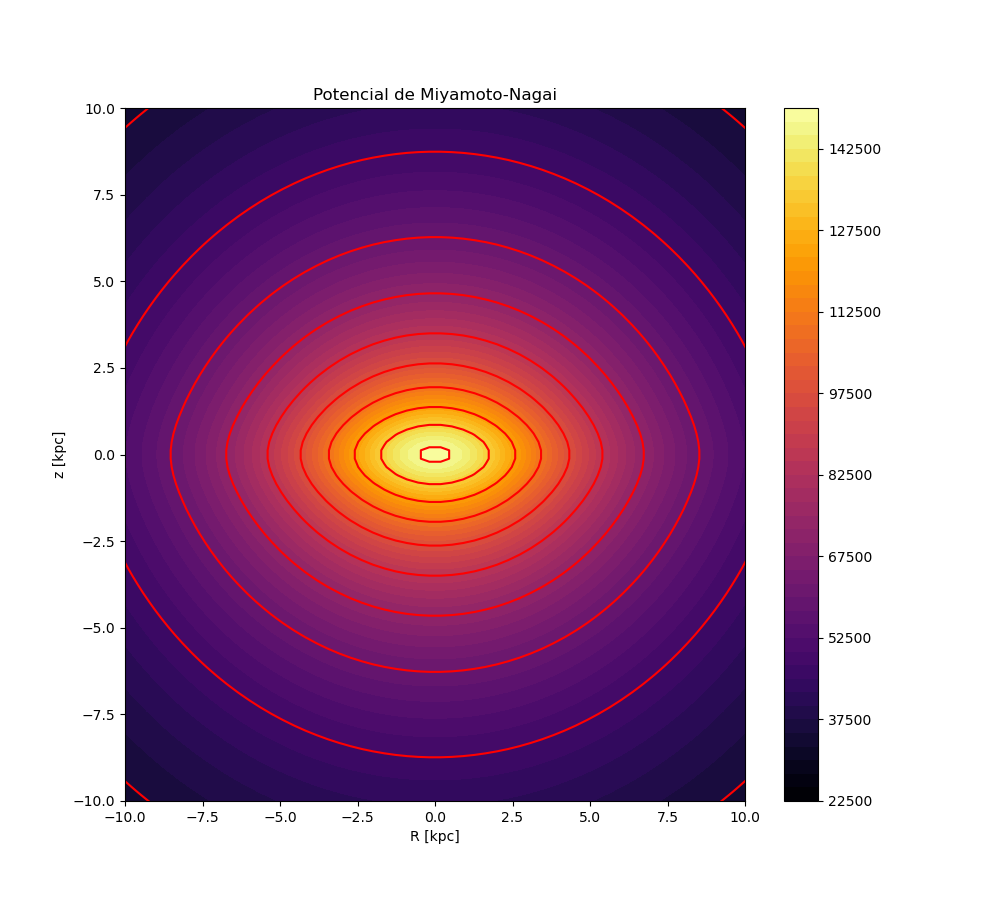
\includegraphics[width=\columnwidth]{../potencial.png}
\caption{Potencial de Miyamoto-Nagai. Como el potencial es definido negativo, en la figura se muestran los contornos de $-\phi(R,z)$ para una razón $b/a=0.25$ con $a=3$ y $M=1.3\times10^{11}~M_\odot$.} \label{fig:MNpot}
\end{figure} 

Este potencial da lugar a una densidad de la forma

\begin{equation}
\rho=\frac{b^2M}{4\pi}\frac{aR^2+(a+3\sqrt{z^2+b^2})(a+\sqrt{z^2+b^2})^2}{[R^2+(a+\sqrt{z^2+b^2})^2]^{5/2}(z^2+b^2)^{3/2}}. \label{eq:MNdens}
\end{equation}

La figura \ref{fig:MNdens} muestra los contornos de este perfil de densidad.

\begin{figure}[h!]
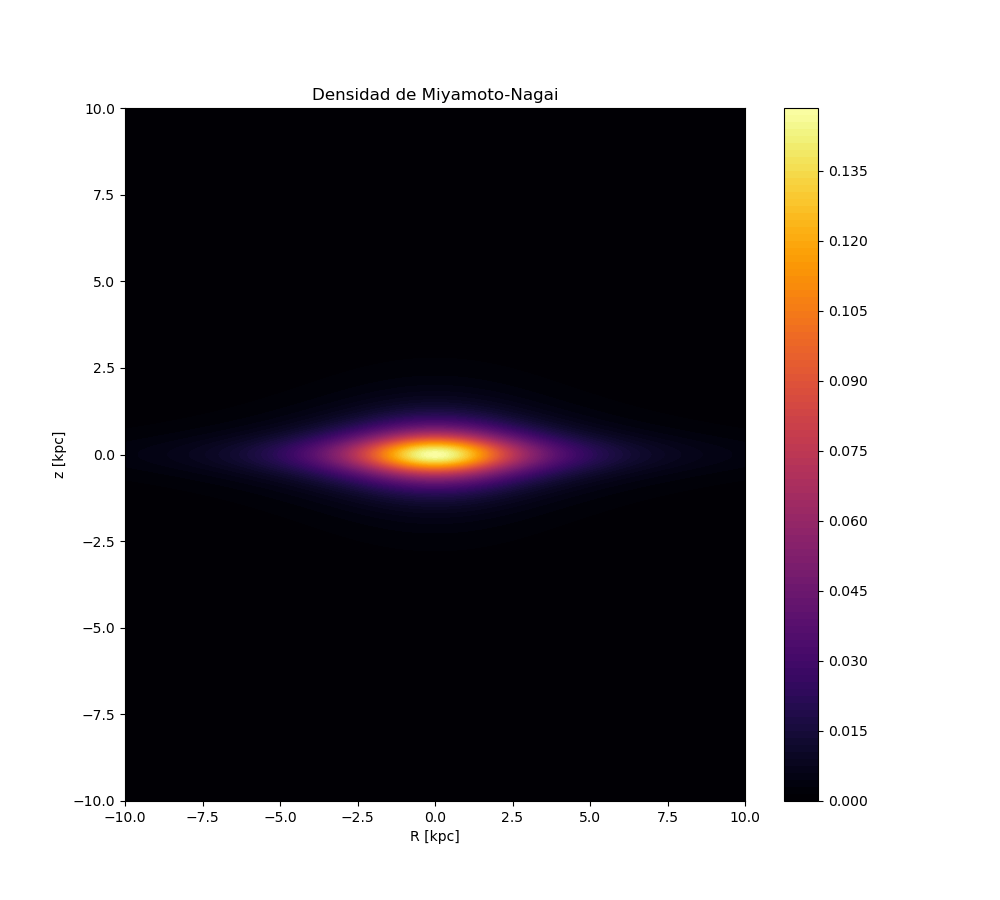
\includegraphics[width=\columnwidth]{../densidad.png}
\caption{Densidad de Miyamoto-Nagai. En la figura se muestran los contornos de $\rho(R,z)$ para una razón $b/a=0.25$ con $a=3~\text{kpc}$ y $M=1.3\times10^{11}~M_\odot$.} \label{fig:MNdens}
\end{figure} 

Los parámetros $a$ y $b$ controlan la forma de la distribución y, por tanto, de la galaxia: si $a=0$, el perfil de Miyamoto-Nagai se reduce a un perfil de Plummer, que tiene simetría esférica; así, mientras más grande es $a$, la forma del disco se aleja más de la de una esfera, esto es, se achata. Por otro lado, si $b=0$, el perfil de Miyamoto-Nagai se tiende al perfil de Kuzmin, que describe discos infinitesimalmente delgados, de manera que $b$ controla el grosor del disco. Para este ejercicio, se escogieron $a$ y $b$ tales que se cumpla que $b/a=0.25$, se escogió a su vez un valor de $a=3~\text{kpc}$, de modo que se está modelando una galaxia relativamente achatada y con un disco considerablemente delgado, en tanto $b=0.75~\text{kpc}$; esto se puede confirmar en la gráfica de la densidad mostrada en la figura \ref{fig:MNdens}. Finalmente, se escogió un valor de $1.3\times10^{11}~M_\odot$ para la masa, teniendo como referencia la galaxia de Andrómeda (M31), pues es este el valor de su masa estelar \cite{Corbelli_2010}.\\

Considérese una órbita en equilibrio en el plano de la galaxia $z=0$. Esta órbita es una circunferencia de radio $R_g$, conocido como \emph{radio guía}, y representa una condición de equilibrio estable para el sistema en tanto $\nabla\phi_{eff}(R_g,0)=\vec{0}$ y $\phi_{eff}(R_g,0)$ es un mínimo del potencial efectivo, definido como:

\begin{equation}
\phi_{eff}(R,z)=\phi(R,z)+\dfrac{L_z^2}{2R^2}. \label{eq:poteff}
\end{equation}

Esto implica que una estrella puede presentar pequeñas oscilaciones en las direcciones radial y vertical en torno a la órbita guía. Expandiendo el potencial efectivo en series de Taylor alrededor de la posición de equilibrio hasta el primer orden no nulo, se encuentra que:

\begin{equation}
\phi_{eff}(R,z)\approx \dfrac{1}{2}\kappa^2x^2+\dfrac{1}{2}\nu^2z^2, \label{eq:potOA}
\end{equation}

que es el potencial de dos osciladores armónicos desacoplados, donde $x$ y $z$ son las pequeñas perturbaciones a la posición de equilibrio y 

\begin{align}
\kappa^2=\left.\dfrac{\partial^2\phi_{eff}}{\partial R^2}\right|_{(R_g,0)}=\left.\dfrac{\partial^2\phi}{\partial R^2}\right|_{(R_g,0)}+\dfrac{3L_z^2}{R_g^4}, \label{eq:fepi}\\
\nu^2=\left.\dfrac{\partial^2\phi_{eff}}{\partial z^2}\right|_{(R_g,0)}=\left.\dfrac{\partial^2\phi}{\partial z^2}\right|_{(R_g,0)}. \label{eq:fvert}
\end{align}

Estas cantidades se conocen como \emph{frecuencia de epiciclo} y \emph{frecuencia vertical}, respectivamente. Adicionalmente, en la posición de equilibrio se satisface que

\begin{equation}
\left.\dfrac{\partial\phi_{eff}}{\partial R}\right|_{(R_g,0)}=\left.\dfrac{\partial\phi}{\partial R}\right|_{(R_g,0)}-\dfrac{L_z^2}{R_g^3}=0. \label{eq:eq}
\end{equation}

Reemplazando el resultado \ref{eq:eq} en la frecuencia de epiciclo \ref{eq:fepi} se puede obtener una expresión para $\kappa^2$ en términos de las derivadas del potencial:

\begin{equation}
\kappa^2=\left.\dfrac{\partial^2\phi}{\partial R^2}\right|_{(R_g,0)}+\dfrac{3}{R_g}\left.\dfrac{\partial\phi}{\partial R}\right|_{(R_g,0)}. \label{eq:fepi2}
\end{equation}

Para el potencial de Miyamoto-Nagai, las derivadas radiales del potencial están dadas por:

\begin{align}
\dfrac{\partial\phi}{\partial R}=\frac{G M R}{\left(R^2+\left(a+\sqrt{b^2+z^2}\right)^2\right)^{3/2}}\label{eq:dphidR},\\
\dfrac{\partial^2\phi}{\partial R^2}=\frac{G M \left(a^2+b^2-2 R^2+z^2+2 a \sqrt{b^2+z^2}\right)}{\left(R^2+\left(a+\sqrt{b^2+z^2}\right)^2\right)^{5/2}}.\label{eq:d2phidR2}
\end{align}

Al evaluar en la posición de equilibrio, teniendo en cuenta que $b,R_g>0$, y sustituir en \ref{eq:fepi2}, se obtiene que la frecuencia de epiciclo es

\begin{equation}
\kappa^2(R_g)=\frac{G M \left(4 (a+b)^2+R_g^2\right)}{\left((a+b)^2+R_g^2\right)^{5/2}}. \label{eq:fepiMN}
\end{equation}

Similarmente, la segunda derivada del potencial respecto a $z$ es dada por:

\begin{align}
\dfrac{\partial^2\phi}{\partial z^2}=-\frac{3 G M z^2 \left(a+\sqrt{b^2+z^2}\right)^2}{\left(b^2+z^2\right) \left(R^2+\left(a+\sqrt{b^2+z^2}\right)^2\right)^{5/2}}+\nonumber\\+\frac{G
M z^2}{\left(b^2+z^2\right) \left(R^2+\left(a+\sqrt{b^2+z^2}\right)^2\right)^{3/2}}-\nonumber\\-\frac{G M z^2 \left(a+\sqrt{b^2+z^2}\right)}{\left(b^2+z^2\right)^{3/2}
\left(R^2+\left(a+\sqrt{b^2+z^2}\right)^2\right)^{3/2}}+\nonumber\\+\frac{G M \left(a+\sqrt{b^2+z^2}\right)}{\sqrt{b^2+z^2} \left(R^2+\left(a+\sqrt{b^2+z^2}\right)^2\right)^{3/2}}.\label{eq:d2phidz2}
\end{align}

Sin embargo, es fácil ver que tres de los términos de \ref{eq:d2phidz2} se anulan al evaluar en la órbita guía, dando lugar a la expresión para la frecuencia vertical:

\begin{equation}
\nu^2(R_g)=\frac{(a+b) G M}{b \left((a+b)^2+R^2\right)^{3/2}} \label{eq:fvertMN}
\end{equation}

Nótese que, si se escribe $4(a+b)^2=3(a+b)^2+(a+b)^2$, \ref{eq:fepiMN} se puede descomponer en dos términos: el primero proporcional a $\left((a+b)^2+R_g^2\right)^{-5/2}$ y el segundo proporcional a $\left((a+b)^2+R_g^2\right)^{-3/2}$, de modo que al tomar la derivada con respecto a $R$ de la frecuencia de epiciclo, se encuentra que esta es negativa para todo valor de $R$, esto es, la frecuencia de epiciclo es una función monótonamente decreciente con $R$. Análogamente, la frecuencia vertical es proporcional a $\left((a+b)^2+R_g^2\right)^{-3/2}$ y su derivada es negativa para cualqueir valor de $R$, haciendo de la frecuencia vertical una función monótonamente decreciente. Este comportamiento de las frecuencias tiene sentido pues para órbitas con radio guía pequeño, la fuerza de restitución que soporta el movimiento oscilatorio, y que es provista por el campo gravitacional, es mayor, haciendo que las oscilaciones tengan una frecuencia más alta. La figura \ref{fig:frecs} muestra las frecuencias de epiciclo y vertical en función de la distancia al centro galáctico para órbitas levemente perturbadas del plano galáctico.\\

\begin{figure}[h!]
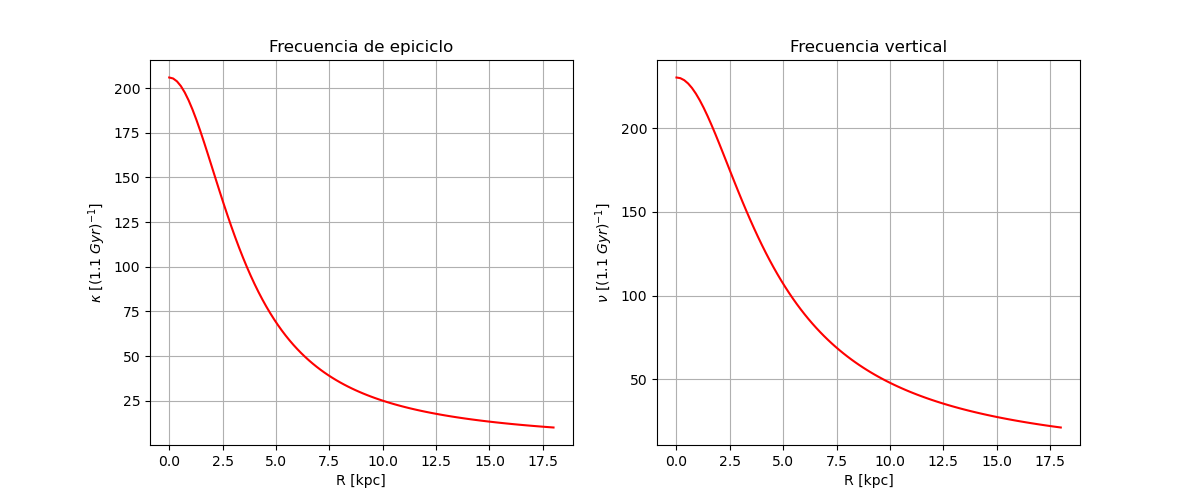
\includegraphics[width=\columnwidth]{../frecuenciasMN.png}
\caption{Frecuencias de epiciclo y vertical para el potencial de Miyamoto-Nagai.} \label{fig:frecs}
\end{figure} 

En las coordenadas $R$ y $z$, las ecuaciones de movimiento son las de un oscilador armónico que oscila alrededor de los puntos de equilibrio, luego las soluciones a dichas ecuaciones son:

\begin{align}
R(t)=R_g+x_0\cos(\kappa t+\psi), \label{eq:OAR}\\
z(t)=z_0\cos(\nu t+\zeta), \label{eq:OAZ}
\end{align}

donde $\psi,\zeta$ son fases arbitrarias y $x_0,z_0$ son las amplitudes de las oscilaciones, que en principio están determinadas por la energía del sistema y deben ser pequeñas. Por otro lado, la primera integral del movimiento azimutal da lugar a $\dot{\varphi}=L_zR(t)^{-2}$, que, al reemplazar \ref{eq:OAR} y usar la aproximación binomial, la ecuación se puede integrar en el tiempo para obtener una expresión general para el ángulo:

\begin{equation}
\varphi(t)=\varphi_0+\Omega_0t-\frac{2x_0}{R_g\kappa}\sin(\kappa t+\psi),\label{eq:azimut}
\end{equation}

donde $\varphi_0$ es una constante de integración arbitraria y $\Omega_0=L_zR_g^{-2}$, que puede escribirse en términos de la derivada del potencial de acuerdo a \ref{eq:eq}. Al combinar entonces estas  ecuaciones, se puede describir por completo el movimiento de una estrella en una órbita casi circular, como se muestra en la figura \ref{fig:orbs}.

\begin{figure}[h!]
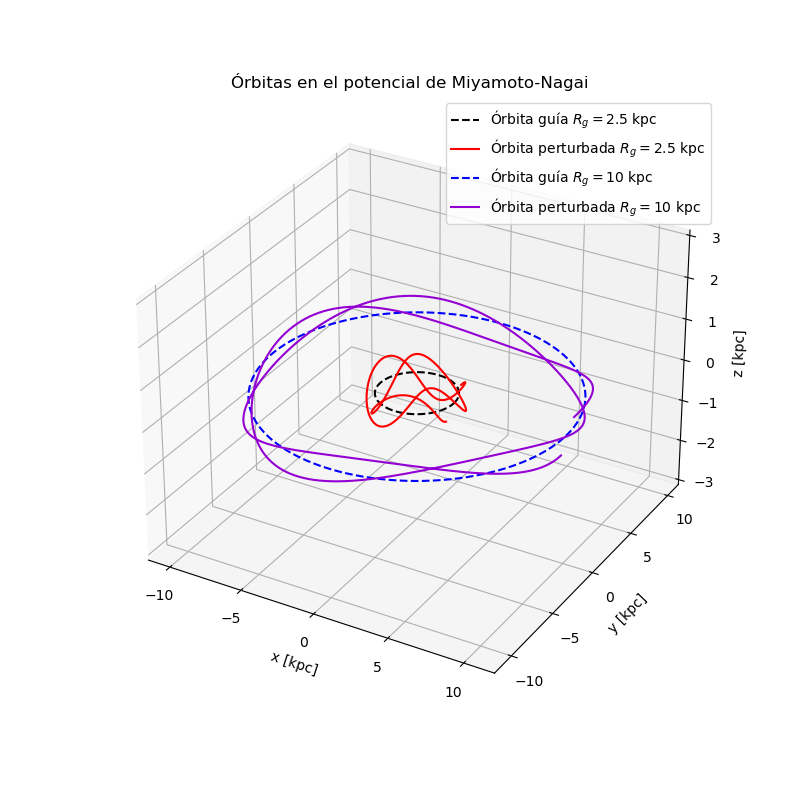
\includegraphics[width=\columnwidth]{../orbitasMN.png}
\caption{Órbitas guía y órbitas perturbadas en el potencial de Miyamoto-Nagai. Se escogieron dos radios guía: 2.5 kpc y 10 kpc para ilustrar el comportamiento de las perturbaciones a distintos radios. Aquí, se escogieron las fases arbitrarias iguales a 0 y las amplitudes iguales a 1 para poder apreciar la oscilación alrededor de la órbita guía. Cada órbita se integra en dos períodos de su respectiva órbita guía.} \label{fig:orbs}
\end{figure} 

\section{Constantes de Oort en el vecindario solar y modelo de la Vía Láctea}

Considérese una estrella en el disco de la galaxia, y supondremos que el Sol está también sobre el disco. Ambas estrellas tienen una velocidad circular en torno al centro de la galaxia como se muestra en la figura \ref{fig:vc}, siendo $\vec{v}_0$ la velocidad circular del Sol y $\vec{v}_c$ la velocidad circular de la estrella.

\begin{figure}[h!]
\centering
\begin{tikzpicture}[dot/.style={circle,draw,fill=black,minimum size=5}]

%\draw[
%  help lines,
%  line width=0.1pt,
%  gray!30,
%] (-3, -3) grid[step={($(0.25, 0.25) - (0, 0)$)}] (3, 3);
%\draw[
%  help lines,
%  line width=0.1pt,
%  gray,
%] (-3, -3) grid[step={($(1, 1) - (0, 0)$)}] (3, 3);

\draw (1,3)--(1,-1) node [midway, right] {$R_0$} --(0,0) node[midway, below] {$d$} --(-1,1) node[left] {$T$}--(1,3)--(0,0) node [midway, right] {$R$};

\draw[mark=*,mark size=4pt,mark options={color=red}] plot coordinates {(1,3)} node [above left] {$C$};
\draw[mark=10-pointed star,mark size=3pt,mark options={color=red}] plot coordinates {(1,-1)} node [below] {$O$};
\draw[mark=10-pointed star,mark size=3pt,mark options={color=red}] plot coordinates {(0,0)} node[below] {$S$};

\draw[-stealth, blue] (1,-1) -- (0,-1) node [midway, below] {$\vec{v}_0$};
\draw[-stealth, blue] (0,0) -- (-1,0.333) node [midway, below] {$\vec{v}_c$};

\end{tikzpicture}

\caption{Movimiento de una estrella $S$ y el Sol $O$ alrededor del centro de la galaxia $C$. El ángulo $\measuredangle COS$ es la longitud galáctica $l$, el ángulo $\measuredangle TCS$ lo denotaremos en lo que sigue como $\alpha$ y el ángulo $\measuredangle SCO$ lo denotaremos como $\beta$. $R_0$ es la distancia del Sol al centro galáctico, $R$ es la distancia de la estrella al centro galáctico y $d$ es la distancia del Sol a la estrella.}\label{fig:vc}
\end{figure} 

Por construcción, las velocidades se pueden descomponer en una componente radial a lo largo de la línea de la visual $\overline{OS}$ y una componente tangencial perpendicular a la línea de la visual. Las componentes radial y tangencial de la velocidad circular de la estrella alrededor del centro galáctico se pueden relacionar con la velocidad radial y tangencial observada, restando las componentes radial y tangencial de la velocidad del Sol, dando lugar a las siguientes expresiones para las velocidades radial y tangencial observadas, $v_r$ y $v_t$, respectivamente:

\begin{align}
v_r = v_c\cos\alpha-v_0\sin l, \label{eq:vr}\\
v_t = v_c\sin\alpha-v_0\cos l. \label{eq:vt}
\end{align}

Manipulando algebraicamente estas expresiones, con ayuda de las relaciones que surgen de la geometría del sistema, es posible obtener una expresión para estas cantidades en el vecindario solar, considerando $\beta\ll 1$:

\begin{align}
v_r \approx Ad\sin 2l, \label{eq:vrap}\\
v_t \approx Ad\cos 2l+Bd, \label{eq:vtap}
\end{align}

donde $A$ y $B$ se conocen como \emph{constantes de Oort}, y se definen como

\begin{align}
A = -\frac{1}{2}\left(\left.\frac{\mathrm{d}v_c}{\mathrm{d}R}\right|_{R_0}-\frac{v_0}{R_0}\right), \label{eq:oortA}\\
B = -\frac{1}{2}\left(\left.\frac{\mathrm{d}v_c}{\mathrm{d}R}\right|_{R_0}+\frac{v_0}{R_0}\right), \label{eq:oortB}
\end{align}

En esta sección se hará una estimación de las constantes de Oort en el vecindario solar a partir de un conjunto de datos observacionales de dos millones de estrellas de la Vía Láctea provistos en las instrucciones del trabajo. Estos datos se almacenaron en un \texttt{DataFrame} de \texttt{pandas} con las siguientes columnas:

\begin{enumerate}
\item ID.
\item Época.
\item Ascención recta [deg].
\item Declinación [deg].
\item Paralaje [arcsec].
\item Movimiento propio [mas/yr].
\item Velocidad radial relativa al Sol [km/s].
\item Longitud galáctica [deg].
\item Latitud galáctica [deg].
\item Distancia al Sol (método 1) [pc].
\item Distancia al Sol (método 2) [pc].
\end{enumerate}

Para el cálculo de $A$ y $B$ fue necesario filtrar los datos, pues es evidente la necesidad de tener datos sobre la velocidad radial de las estrellas para poder ajustar las constantes de Oort, lo que reduce la muestra de dos millones de estrellas a apenas 45165 que tienen la medición de su velocidad radial. Adicional a esto, se hace necesario filtrar las estrellas que están en el vecindario solar, que, de acuerdo a \cite{binney2011galactic}, está entre 1 y 2 kpc si se quieren contar hasta las estrellas de tipo O o B, que son más luminosas pero menos abundantes; así pues, se consideraron las estrellas que se encuentran a una distancia de máximo 1 kpc del Sol como aquellas pertenecientes al vecindario solar, con el fin de obtener posiblemente una muestra representativa con diversos tipos de estrellas, de modo que ahora se tiene una muestra de 16796 estrellas. Finalmente, las ecuaciones \ref{eq:vrap} y \ref{eq:vtap} se obtuvieron teniendo en cuenta la aproximación $\beta\ll 1$, por lo cual se escogieron las estrellas con $\beta<0.01$ para satisfacer este criterio, dejando finalmente una muestra de 1875 estrellas, donde $\beta$ se calculó usando la ley del seno en el triángulo $CSO$ de la figura \ref{fig:vc}, dando como resultado

\begin{equation}
\beta=\arcsin\left(\frac{d\sin l}{R}\right). \label{eq:beta}
\end{equation}

Se omitió el análisis estadístico sobre la representatividad de las muestras sucesivas que se escogieron, pues estas no fueron escogidas de manera aleatoria sino siguiendo criterios muy específicos.\\

La distancia de cada estrella al centro galáctico se obtuvo a partir de sus coordenadas cartesianas con respecto al mismo, que pueden ser obtenidas a partir de las coordenadas galácticas:

\begin{align}
x_* = d\cos b\cos l-8~\text{kpc}, \label{eq:xcg}\\
y_* = d\cos b\sin l, \label{eq:ycg}\\
z_* = d\sin b, \label{eq:zcg}
\end{align}

donde para la coordenada $x_*$ se restó la distancia del Sol al centro galáctico, $R_0=8~\text{kpc}$ \cite{binney2011galactic} para trasladar allí el sistema de referencia, de modo que 

\begin{equation}
R=\sqrt{x_*^2+y_*^2+z_*^2}. \label{eq:Rcg}
\end{equation}

Así entonces se ajustaron los datos de la velocidad radial, distancia y longitud galáctica a la ecuación \ref{eq:vrap} para obtener un valor de A de 

\begin{equation}
A=16.43~\text{km/s/kpc}, \label{eq:A}
\end{equation}

que es comparable con el valor de 14.8 km/s/kpc reportado en la literatura \cite{binney2011galactic}.\\

De las definiciones \ref{eq:oortA} y \ref{eq:oortB} es facil obtener la relación:

\begin{equation}
A-B=\frac{v_0}{R_0}, \label{eq:rel}
\end{equation}

para evitar hacer el ajuste de $B$ con los datos observacionales, pues, si bien la velocidad tangencial observada se puede calcular a partir del movimiento propio, $\mu$, y la distancia del Sol a la estrella, de acuerdo a la ecuación \ref{eq:vtcalc}, los datos solo contienen la magnitud del movimiento propio, no sus componentes, que son necesarias para poder ajustar correctamente la velocidad tangencial a la función armónica de la ecuación \ref{eq:vtap} en tanto son estas componentes las que dan cuenta de la dirección de la velocidad tangencial y proveerán el signo de la velocidad tangencial proyectada en el plano del disco.

\begin{equation}
v_t=\mu d. \label{eq:vtcalc}
\end{equation}

Usando entonces la ecuación \ref{eq:rel}, $v_0=220~\text{km/s}$ y $R_0=8~\text{kpc}$ \cite{binney2011galactic}, se obtiene un valor de $B$ de

\begin{equation}
B=-11.07~\text{km/s/kpc}, \label{eq:B}
\end{equation}

que es comparable con el valor de -12.4 km/s/kpc reportado en la literatura \cite{binney2011galactic}. Estos resultados dejan ver que, con las definiciones teóricas de las constantes de Oort y definiendo apropiadamente el vecindario solar, es suficiente ajustar la velocidad radial de las estrellas contenidas en este para obtener un buen estimativo de las constantes de Oort.\\

Ahora bien, teniendo estos datos, se busca ajustar el disco de la Vía Láctea a un perfil de Miyamoto-Nagai a través de la velocidad circular, definida por:

\begin{equation}
v_c^2(R)=R\left.\frac{\partial \phi}{\partial R}\right|_{z=0}=\frac{GMR^2}{\left((a+b)^2+R^2\right)^{3/2}}. \label{eq:vcMN}
\end{equation}

Para esto, fue necesario obtener la velocidad tangencial usando la ecuación \ref{eq:vtcalc} en las unidades apropiadas para calcular la velocidad circular cuadrática como

\begin{equation}
v_c^2=v_r^2+v_t^2, \label{eq:vc2}
\end{equation}

por lo que fue nuevamente necesario escoger las estrellas que tuvieran datos de velocidad radial. Ajustando los datos a la ecuación \ref{eq:vcMN} a la velocidad circular de Miyamoto-Nagai con los parámetros escogidos en la sección anterior, es decir, $a=3~\text{kpc}$ y $b=0.25a$, esto da lugar a un valor de la masa del disco de 

\begin{equation}
M=(2.68\pm 0.03)\times10^{10}M_\odot, \label{eq:mass}
\end{equation}

y a un ajuste como el que se muestra en la figura \ref{fig:fit}.

\begin{figure}[h!]
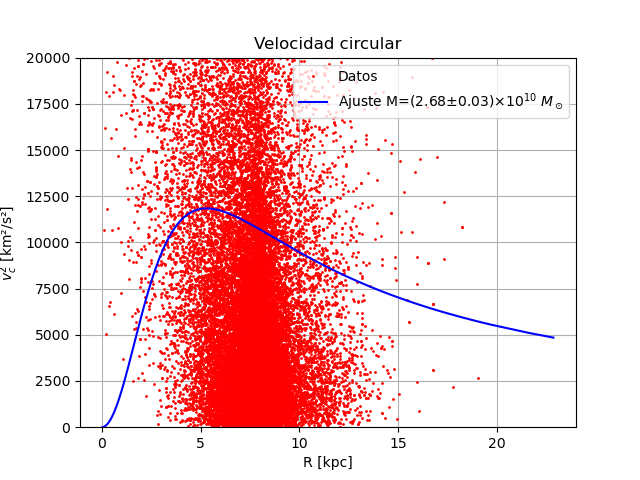
\includegraphics[width=\columnwidth]{../ajusteMW.png}
\caption{Ajuste de las velocidades circulares cuadráticas a la curva de rotación de Miyamoto-Nagai.} \label{fig:fit}
\end{figure} 

Es evidente que, aún si la calidad del ajuste a los datos no es muy buena de cuenta de la alta dispersión de los mismos, se puede obtener un valor de la masa de al menos el mismo orden de magnitud de los $\simeq 6\times10^{10} M_\odot$ reportados en la literatura \cite{carroll2017introduction}, sin embargo, al tratar de ajustar también los parámetros $a$ y $b$, se obtienen valores negativos, lo cual no tiene sentido físico, en tanto $a$ y $b$ controlan la geometría del potencial y representan escalas de distancia. Este resultado puede mejorar si se filtra adecuadamente el conjunto de datos para tener en consideración únicamente las estrellas más cercanas al plano del disco.

\section{Halo de materia oscura}

El halo de materia oscura es un sistema con simetría esférica, por lo que se ha de modelar con un potencial únicamente dependiente de $r$, la distancia al origen de coordenadas. Se escogió entonces un \emph{perfil de Hernquist}, dado por la ecuación \ref{eq:Hpot} \cite{binney2011galactic}

\begin{equation}
\phi_H(r)=-\frac{G M_h}{r+\alpha }. \label{eq:Hpot}
\end{equation}

Se escogió este potencial porque, dependiendo del valor que se escoja para $\alpha$, el perfil de Hernquist puede modelar satisfactoriamente un halo de materia oscura de masa $M_h$. Esta escogencia supone una ventaja ante el perfil de Navarro-Frenk-White (NFW) en el cálculo de la masa total, y es que la masa del perfil de NFW diverge al integrar la densidad hasta el infinito \cite{binney2011galactic,carroll2017introduction}, por lo que se debe truncar en el radio virial del halo, lo que supondría un parámetro más en el ajuste del modelo. Inicialmente, se escogieron como parámetros del modelo $M_h=1.2\times 10^{12}M_\odot$, que corresponde a la masa del halo de materia oscura de Andrómeda \cite{Corbelli_2010} y $\alpha=50~\text{kpc}$, considerando que $\alpha$ representa una escala radial para el halo de materia oscura, que en principio debe extenderse muy por fuera del disco, por tanto, hemos de esperar que su tamaño característico sea mucho más grande.\\

Dado que las frecuencias de epiciclo y vertical cuadráticas dependen únicamente de las derivadas del potencial, y la derivada es un operador lineal, la superposición de los dos potenciales resulta entonces en la suma de las frecuencias de epiciclo y vertical cuadráticas para ambos potenciales. En coordenadas cilíndricas, el potencial de Hernquist se puede escribir como

\begin{equation}
\phi_H(R,z)=-\frac{G M_h}{\sqrt{R^2+z^2}+\alpha }. \label{eq:Hpotcil}
\end{equation}

Así pues, las contribuciones a las frecuencias cuadráticas están dadas por:

\begin{align}
\kappa^2_H=\frac{G (R_g+3 \alpha ) M_h}{R_g (R_G+\alpha )^3},\label{eq:fepih}\\
\nu^2_H=\frac{G M_h}{R_g (R_g+\alpha )^2}. \label{eq:fverth}
\end{align}

Y las frecuencias totales están dadas por las ecuaciones \ref{eq:fepiMN}, \ref{eq:fvertMN}, \ref{eq:fepih} y \ref{eq:fverth}

\begin{align}
\kappa_{tot}=\sqrt{\kappa^2+\kappa^2_H}, \label{eq:fepit}\\
\nu_{tot}=\sqrt{\nu^2+\nu^2_H}, \label{eq:fvertt}
\end{align}

Nótese que tanto $\kappa^2_H$ como $\nu^2_H$ son proporcionales a $\alpha^{-2}$, por lo que, al tener un valor de $\alpha$ tan grande para el halo de materia oscura, estas contribuciones no han de ser significativas para las óribtas en general, como se muestra en la figura \ref{fig:frecscorr}, provocando solamente una ligera desviación de las órbitas que se producen solo con el potencial del disco, como se muestra en la figura \ref{fig:orbscorr}. La contribución del potencial de Hernquist con estas carcterísticas a las frecuencias totales se vuelve significativa para valores pequeños del radio guía, pues mientras las frecuencias del potencial de Miyamoto-Nagai tienden a valores constantes cuando $R_g\to0$, las frecuencias del potencial de Hernquist divergen, haciendo que la contribución no sea despreciable.

\begin{figure}[h!]
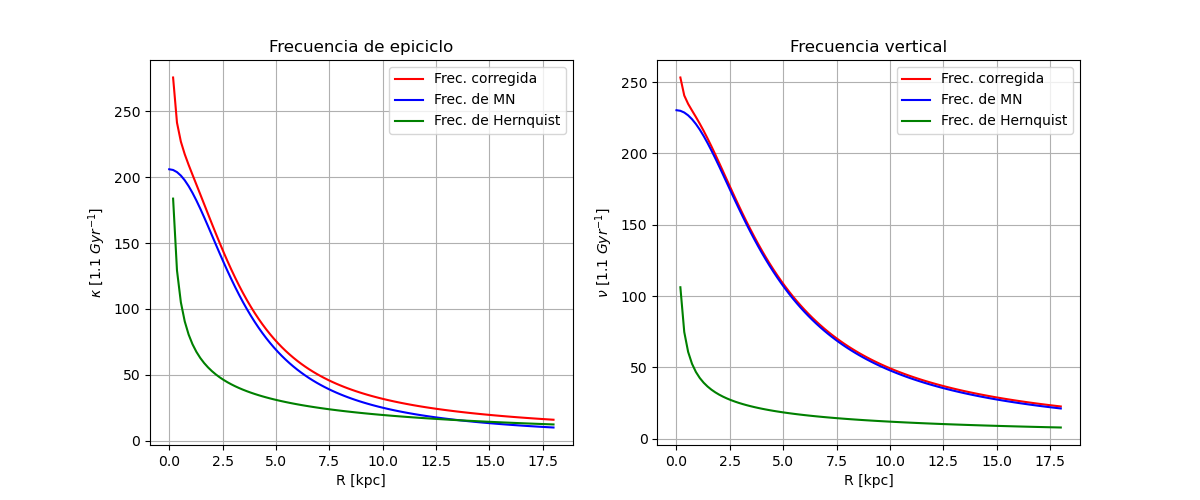
\includegraphics[width=\columnwidth]{../frecuenciascorregidas.png}
\caption{Frecuencias de epiciclo y vertical de los perfiles de Miyamoto-Nagai, Hernquist y total.} \label{fig:frecscorr}
\end{figure} 

\begin{figure}[h!]
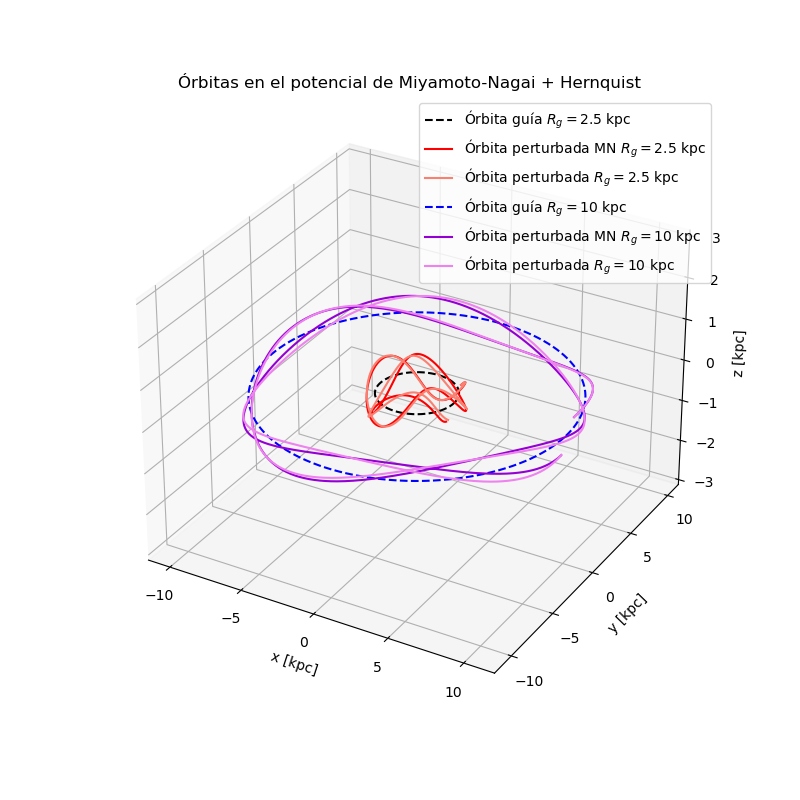
\includegraphics[width=\columnwidth]{../orbitascorregidas.png}
\caption{Órbitas guía y órbitas perturbadas en el potencial de Miyamoto-Nagai y en el potencial total.  Cada órbita se integra en dos períodos de su respectiva órbita guía. Se pone en evidencia entonces que agregar el potencial de un halo de materia oscura con $M_h=1.2\times10^{12}M_\odot$ y $\alpha=50~\text{kpc}$ produce órbitas muy parecidas a las del potencial de Miyamoto-Nagai.} \label{fig:orbscorr}
\end{figure} 

Se desea entonces ajustar los datos de la Vía Láctea a la curva de rotación de la superposición de los dos perfiles que, nuevamente a causa de la linealidad de la derivada, es la suma de las velocidades circulares cuadráticas correspondientes a ambos perfiles:

\begin{equation}
v_{c,tot}^2=G R \left(\frac{M R}{\left((a+b)^2+R^2\right)^{3/2}}+\frac{M_h}{(R+\alpha )^2}\right). \label{eq:vctot}
\end{equation}

Esto da lugar a un valor de la masa del halo de materia oscura de $M_h=(9.6\pm0.1)\times10^9 M_\odot$ y un valor de $\alpha$ de $(0.067\pm0.004)$ kpc. Estos valores no se corresponden con la realidad física de una galaxia de disco, pues la masa del halo de materia oscura de la Vía Láctea es $1.9\times10^{12}M_\odot$ \cite{carroll2017introduction}, por lo que un desfase de alrededor de dos órdenes de magnitud no es aceptable para el valor experimental. Por otro lado, el valor de $\alpha$, que da cuenta del tamaño del halo, indica que la materia oscura está muy concentrada en la región central de la galaxia, cuando se ha observado que este se extiende mucho más allá del disco, pues tiene una escala radial de 170 kpc \cite{carroll2017introduction}. En la figura \ref{fig:halo} se muestra el ajuste.

\begin{figure}[h!]
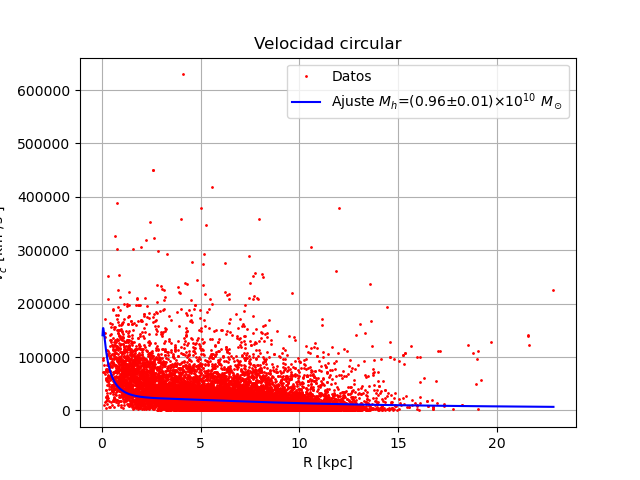
\includegraphics[width=\columnwidth]{../ajusteMWhalo.png}
\caption{Ajuste de las velocidades circulares cuadráticas a la curva de rotación de Miyamoto-Nagai + Hernquist.} \label{fig:halo}
\end{figure} 

En la gráfica se observa además que la velocidad circular decrece con $R$ en lugar de tender a un valor constante, como se esperaría de una galaxia real. El ajuste podría mejorarse potencialmente teniendo datos de la valocidad radial de más estrellas, pues los que se proveen son de una distribución de estrellas centrada en el Sol y relativamente cercanas al disco. De conocer la velocidad radial de estrellas pertenecientes al halo estelar, se podría en principio mejorar la calidad del ajuste y obtener un valor de la masa del halo más cercano al medido a través de las observaciones.

\bibliographystyle{abbrv} 
\bibliography{example.bib}

%% else use the following coding to input the bibitems directly in the
%% TeX file.

%%\begin{thebibliography}{00}

%% \bibitem[Author(year)]{label}
%% For example:

%% \bibitem[Aladro et al.(2015)]{Aladro15} Aladro, R., Martín, S., Riquelme, D., et al. 2015, \aas, 579, A101


%%\end{thebibliography}

\end{document}

\endinput
%%
%% End of file `elsarticle-template-harv.tex'.
